\chapter*{První kroky v~systému}

\section*{Rozkoukáváme se}
Máme před sebou prostředí GNOME Shell. Klíčovým místem pro nás je už zmíněný levý horní roh (tlačítko \emph{Činnosti}), přes který se dostaneme k~vlevo umístěnému menu s~oblíbenými aplikacemi. Stačí do něj najet myší (nebo stisknout levou klávesu \uv{Super}, \uv{Start}, \uv{Meta}, nebo jak ji sami znáte). Jak se dostat ke všem aplikacím? V~menu nalezneme zcela dole ikonu se sadou čtverců \emph{Zobrazit aplikace}. Klikneme na ni a nyní máme aplikace přehledně vyskládané před sebou. Prostředí je velmi intuitivní. Znáte název aplikace? Nebo jen pár prvních písmen? Pak stačí začít psát (nebo použít vyhledávací pole zcela nahoře). Vyhledávání ale neprobíhá pouze mezi aplikacemi, hledá se i mezi kontakty, soubory, možnostmi nastavení a dalšími prvky.

\section*{Pojďme o~něco hlouběji}
Na co se dále zaměřit při běžné práci v~\emph{GNOME}? Předně si všimněte, že okna mají pouze tlačítko pro zavření. Proč je tomu tak, si vysvětlíme při popisu dalšího režimu, minimalizace v~prostředí \emph{GNOME} totiž postrádá smysl a maximalizovat okno lze tažením k~horní hraně obrazovky nebo poklikáním na lištu okna. Úkolem prostředí v~tomto režimu je co nejméně překážet, proto je zobrazen pouze horní panel. Na následujícím obrázku si vysvětlíme hlavní prvky tohoto režimu.

\begin{figure}[t]
\begin{center}
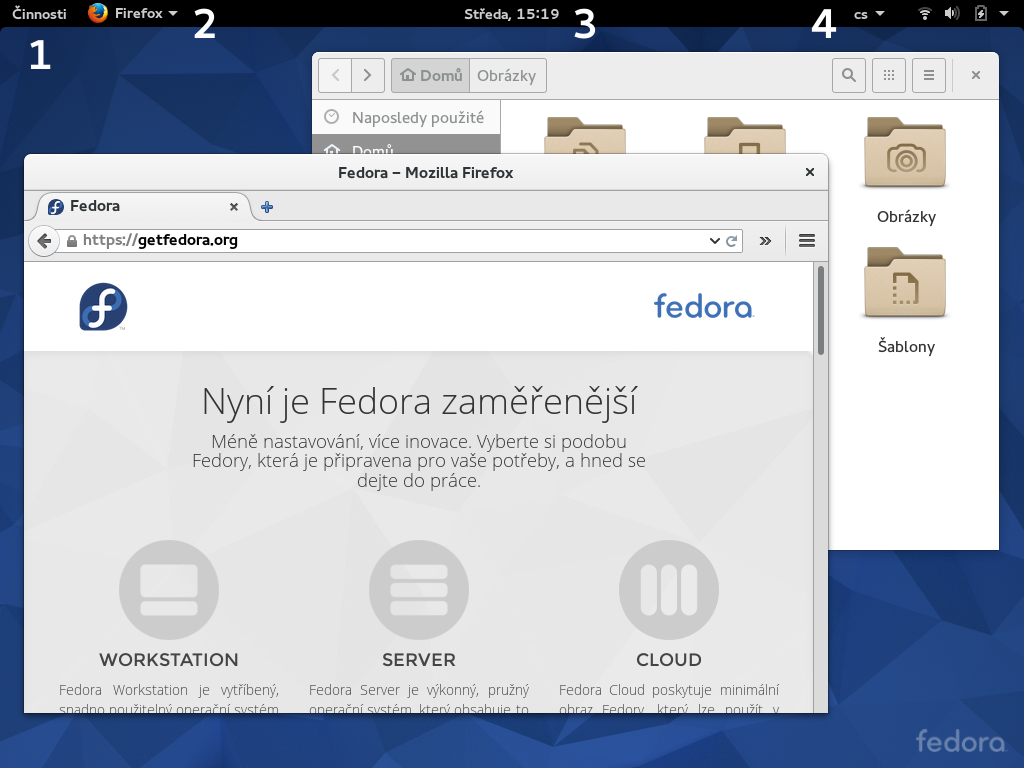
\includegraphics[width=\textwidth]{img/shell-a}
\captionbelow{shell-a.} \label{fig:shell-a}
\end{center}
\end{figure}

\begin{enumerate}
\item\emph{Činnosti} -- jde o~už výše zmíněný prvek, který slouží pro přepnutí do režimu \emph{Činnosti}, jenž je detailněji popsán níže. Je to výchozí bod, přes který se dostaneme k~většině úkonů, které chceme v~systému provádět.

\begin{figure}[t]
\begin{center}
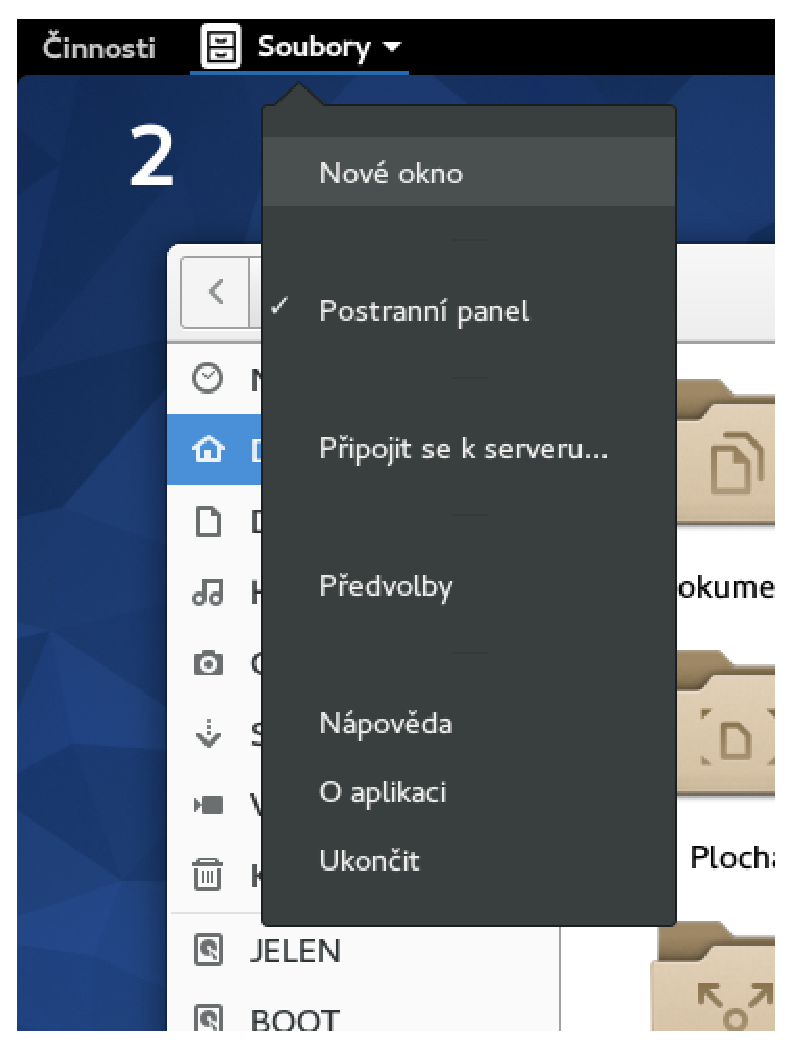
\includegraphics[width=\textwidth]{img/menu-aplikace}
\captionbelow{menu-aplikace.} \label{fig:menu-aplikace}
\end{center}
\end{figure}

\item\emph{Nabídka aplikace} -- pod ikonou momentálně aktivní aplikace naleznete nabídku, která se týká aplikace jako celku (nastavení aplikace, o~aplikaci apod.). Nabídky, které se týkají jednotlivých oken, se nalézají přímo v~okně aplikace. Ne každá aplikace tuto nabídku má. Pokud ji nemá, naleznete pod tímto tlačítkem pouze volbu \emph{Ukončit}.


\begin{figure}[t]
\begin{center}
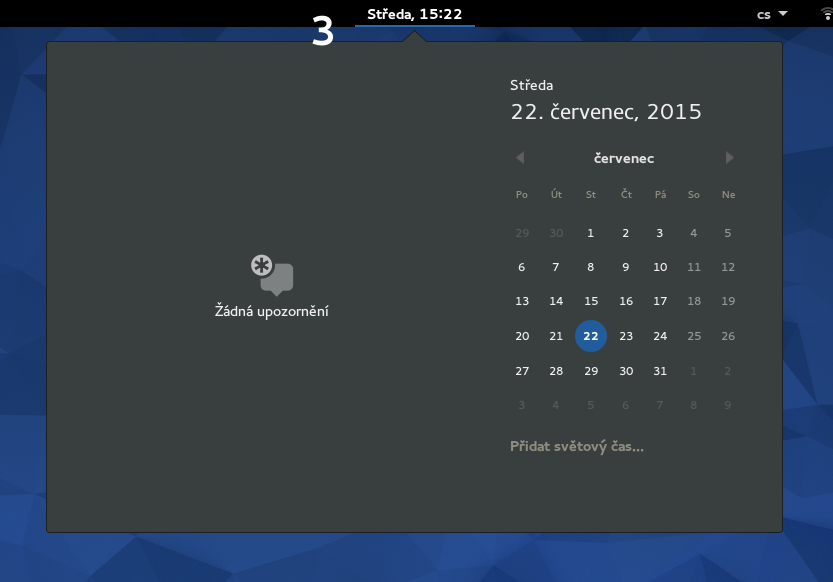
\includegraphics[width=\textwidth]{img/kalendar}
\captionbelow{kalendar.} \label{fig:kalendar}
\end{center}
\end{figure}


\item\emph{Hodiny a kalendář} -- pod zobrazením aktuálního dne a času naleznete kalendář a zmeškaná upozornění. Pokud využíváte jednu z~aplikací, které využívají kalendářový backend \emph{GNOME} (např. \emph{Evolution}), zobrazí se zde i události, které jste v~těchto aplikacích do kalendáře dříve uložili.

\begin{figure}[t]
\begin{center}
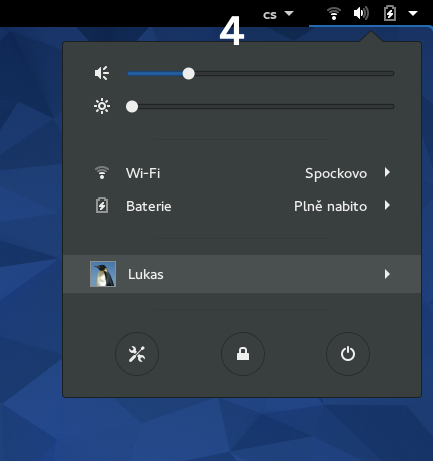
\includegraphics[width=\textwidth]{img/menu}
\captionbelow{menu.} \label{fig:menu}
\end{center}
\end{figure}

\item\emph{Nabídka uživatele} -- v~pravém horním rohu jsou k~dispozici nejdůležitější indikátory (připojení, zvuk, baterie atd.). Po kliknutí na ně se zobrazí nabídka, v~níž můžete nastavit hlasitost, úroveň jasu, připojení k~internetu, bluetooth a další věci. Třetí část nabídky obsahuje vaše jméno s~možnostmi odhlášení se nebo přepnutí do jiného uživatelského účtu. Zcela dole naleznete tři ikony. Ikona nalevo spouští nastavení systému, ta prostřední zamyká obrazovku a ikona napravo vám nabídne restartování nebo vypnutí systému.
\end{enumerate}

\begin{figure}[t]
\begin{center}
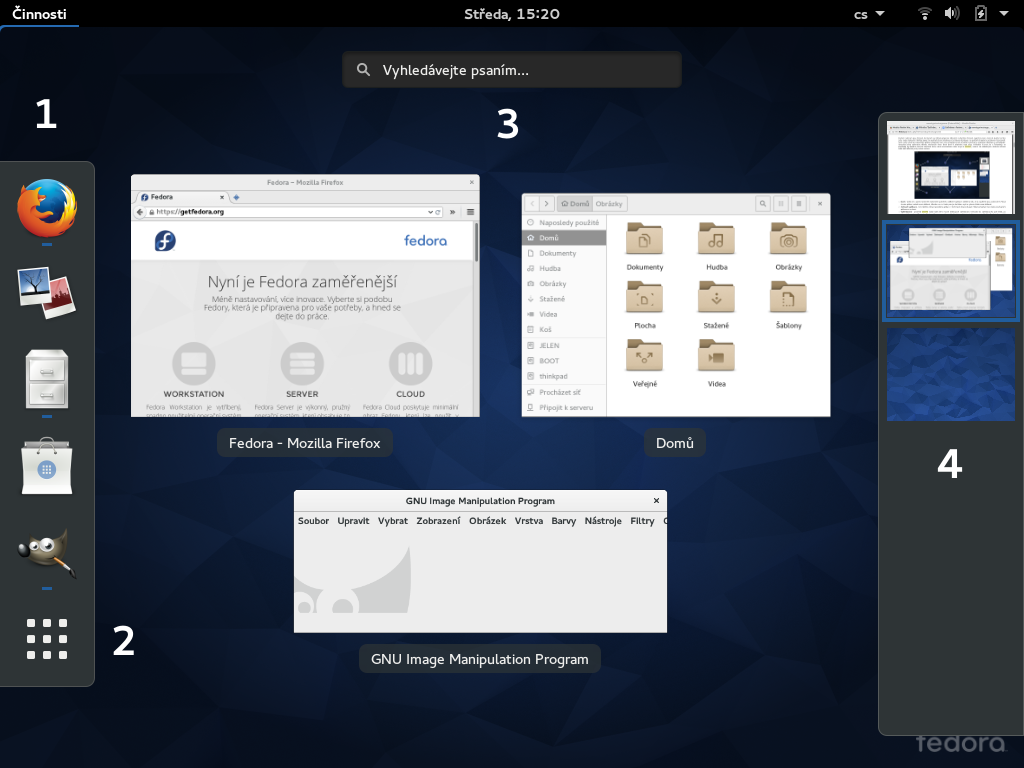
\includegraphics[width=\textwidth]{img/shell-b}
\captionbelow{shell-b.} \label{fig:shell-b}
\end{center}
\end{figure}

\section*{K~čemu slouží \emph{Činnosti}?}
Tento režim je určen pro spouštění aplikací, přepínání mezi nimi, přepínání mezi virtuálními plochami, organizaci desktopu a vyhledávání. Uprostřed obrazovky naleznete náhledy otevřených oken, které slouží k~přepínání mezi aplikacemi. Vzhledem k~tomu, že v~\emph{Činnostech} se poskládají do dlaždice všechna otevřená okna, nemá minimalizace oken smysl a, jak již bylo zmíněno, \emph{GNOME} ji nezná. Na následujícím obrázku můžete vidět další důležité prvky tohoto režimu

\begin{figure}[t]
\begin{center}
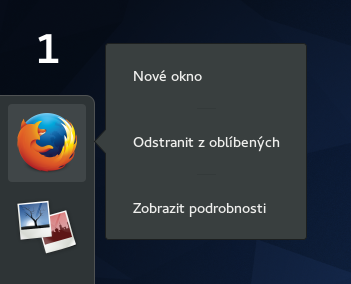
\includegraphics[width=\textwidth]{img/dash-b}
\captionbelow{dash-b.} \label{fig:dash-b}
\end{center}
\end{figure}

\begin{enumerate}
\item \emph{Dash} -- jedná se o~panel (\uv{menu}), na kterém naleznete spuštěné a oblíbené aplikace. Odlišíte je tak, že ty spuštěné jsou výrazně podtržené. Pokud chcete aplikaci zařadit mezi oblíbené, klikněte na ni v~Dashi pravým tlačítkem myši a vyberte \emph{Přidat mezi oblíbené}.

\begin{figure}[t]
\begin{center}
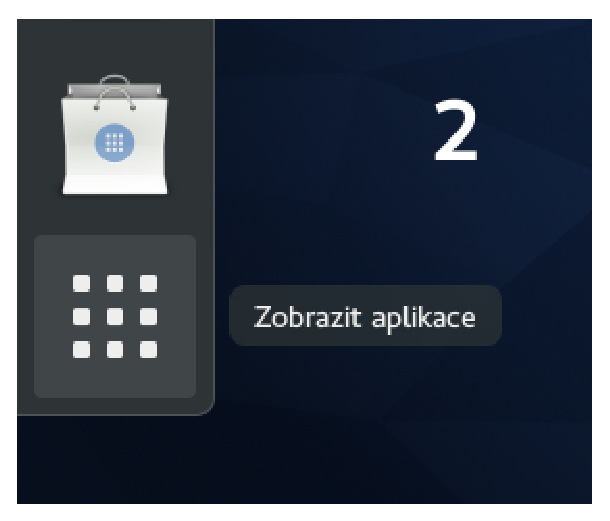
\includegraphics[width=\textwidth]{img/dash-a}
\captionbelow{dash-a.} \label{fig:dash-a}
\end{center}
\end{figure}

\item \emph{Zobrazit aplikace} -- opět již zmíněný prvek. Toto tlačítko zobrazí spouštěče aplikací. V~dolní části obrazovky pak můžete přepínat mezi často používanými aplikacemi a všemi aplikacemi.

\begin{figure}[t]
\begin{center}
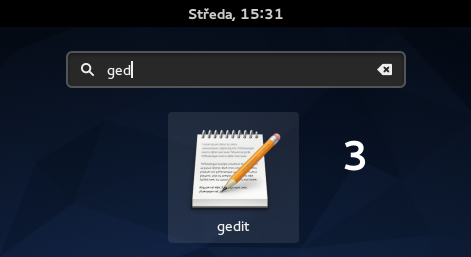
\includegraphics[width=\textwidth]{img/vyhledavani}
\captionbelow{vyhledavani.} \label{fig:vyhledavani}
\end{center}
\end{figure}

\item \emph{Vyhledávání} -- prostředí \emph{GNOME} nabízí také velmi mocné desktopové vyhledávání. Nemusíte do vyhledávacího pole klikat, po přepnutí do režimu \emph{Činnosti} můžete začít rovnou psát a vyhledávání se aktivuje. Jedná se o~nejrychlejší způsob, jak spouštět aplikace. Kromě nich ale můžete vyhledávat také dokumenty, obrázky, virtuální stroje, aplikace k~instalaci, kontakty, atd. Nebo také provádět jednoduché výpočty. Co se má v~\emph{Činnostech} vyhledávat, můžete nastavit v~systémových nastaveních pod položkou \emph{Hledání}.

\item \emph{Virtuální plochy} -- na levé straně můžeme najít náhledy virtuálních ploch, kterých lze mít více, aniž by bylo nutné mít více monitorů. Slouží k~organizaci oken a aplikací. \emph{GNOME} nemá fixní počet ploch. Naopak, jejich počet je dynamický. Je jich vždycky tolik, na kolika z~nich máte aktuálně umístěná okna, a jednu prázdnou navíc, která je připravená k~použití. Když na ni přetáhnete okno, vytvoří se další prázdná a naopak. Přetahovat okna mezi plochami můžete přímo v~náhledech, případně můžete přetáhnout náhled ze středu obrazovky do jednoho z~náhledů. Přepínat mezi virtuálními plochami můžete také přímo v~pracovním režimu pomocí klávesové zkratky $\keystroke{Ctrl}+\keystroke{Alt}+\keystroke{šipka $\uparrow$}\,/\,\keystroke{šipka $\downarrow$}$.

\item \emph{Náhledy otevřených oken} -- slouží k~přehledu o~tom, jaká okna máte otevřená, a také k~přepínání mezi nimi. Přepnutí do vybraného okna provedete najetím myši na okno a kliknutím. Mezi okny můžete přepínat také klávesami. Stačí po přepnutí do \emph{Činností} stisknout klávesu $\keystroke{šipka $\downarrow$}$ a potom pomocí šipek navigovat mezi okny. Přepnutí do vybraného okna provedete klávesou $\keystroke{Enter}$.
\end{enumerate}

\section*{Základní nastavení}
\emph{Uživatelská a systémová nastavení} Fedory nalezneme tak, že stejně jako u~dříve popsaného způsobu napíšeme slovo \uv{nastavení}, nebo přes samopopisnou ikonu v~menu na liště zcela vpravo nahoře. Nastavení jsou členěna do přehledných kategorií (\emph{Osobní}, \emph{Hardware} a \emph{Systém}), kde je možné konfigurovat vše od uživatelských účtů, přes pozadí plochy, až po tiskárny. Naprostá většina běžné konfigurace bude probíhat právě zde. Aplikace umožňuje i propojení s~množstvím online účtů, tedy s~cloudovými službami, ať už používáte ownCloud, Google, Facebook a další. Takto přidaný účet umožní přístup k~službám a datům daného poskytovatele a ostatním aplikacím. Používáte online chat? Potřebujete kontakty? Nic už není nutné zadávat znovu.


\begin{figure}[t]
\begin{center}
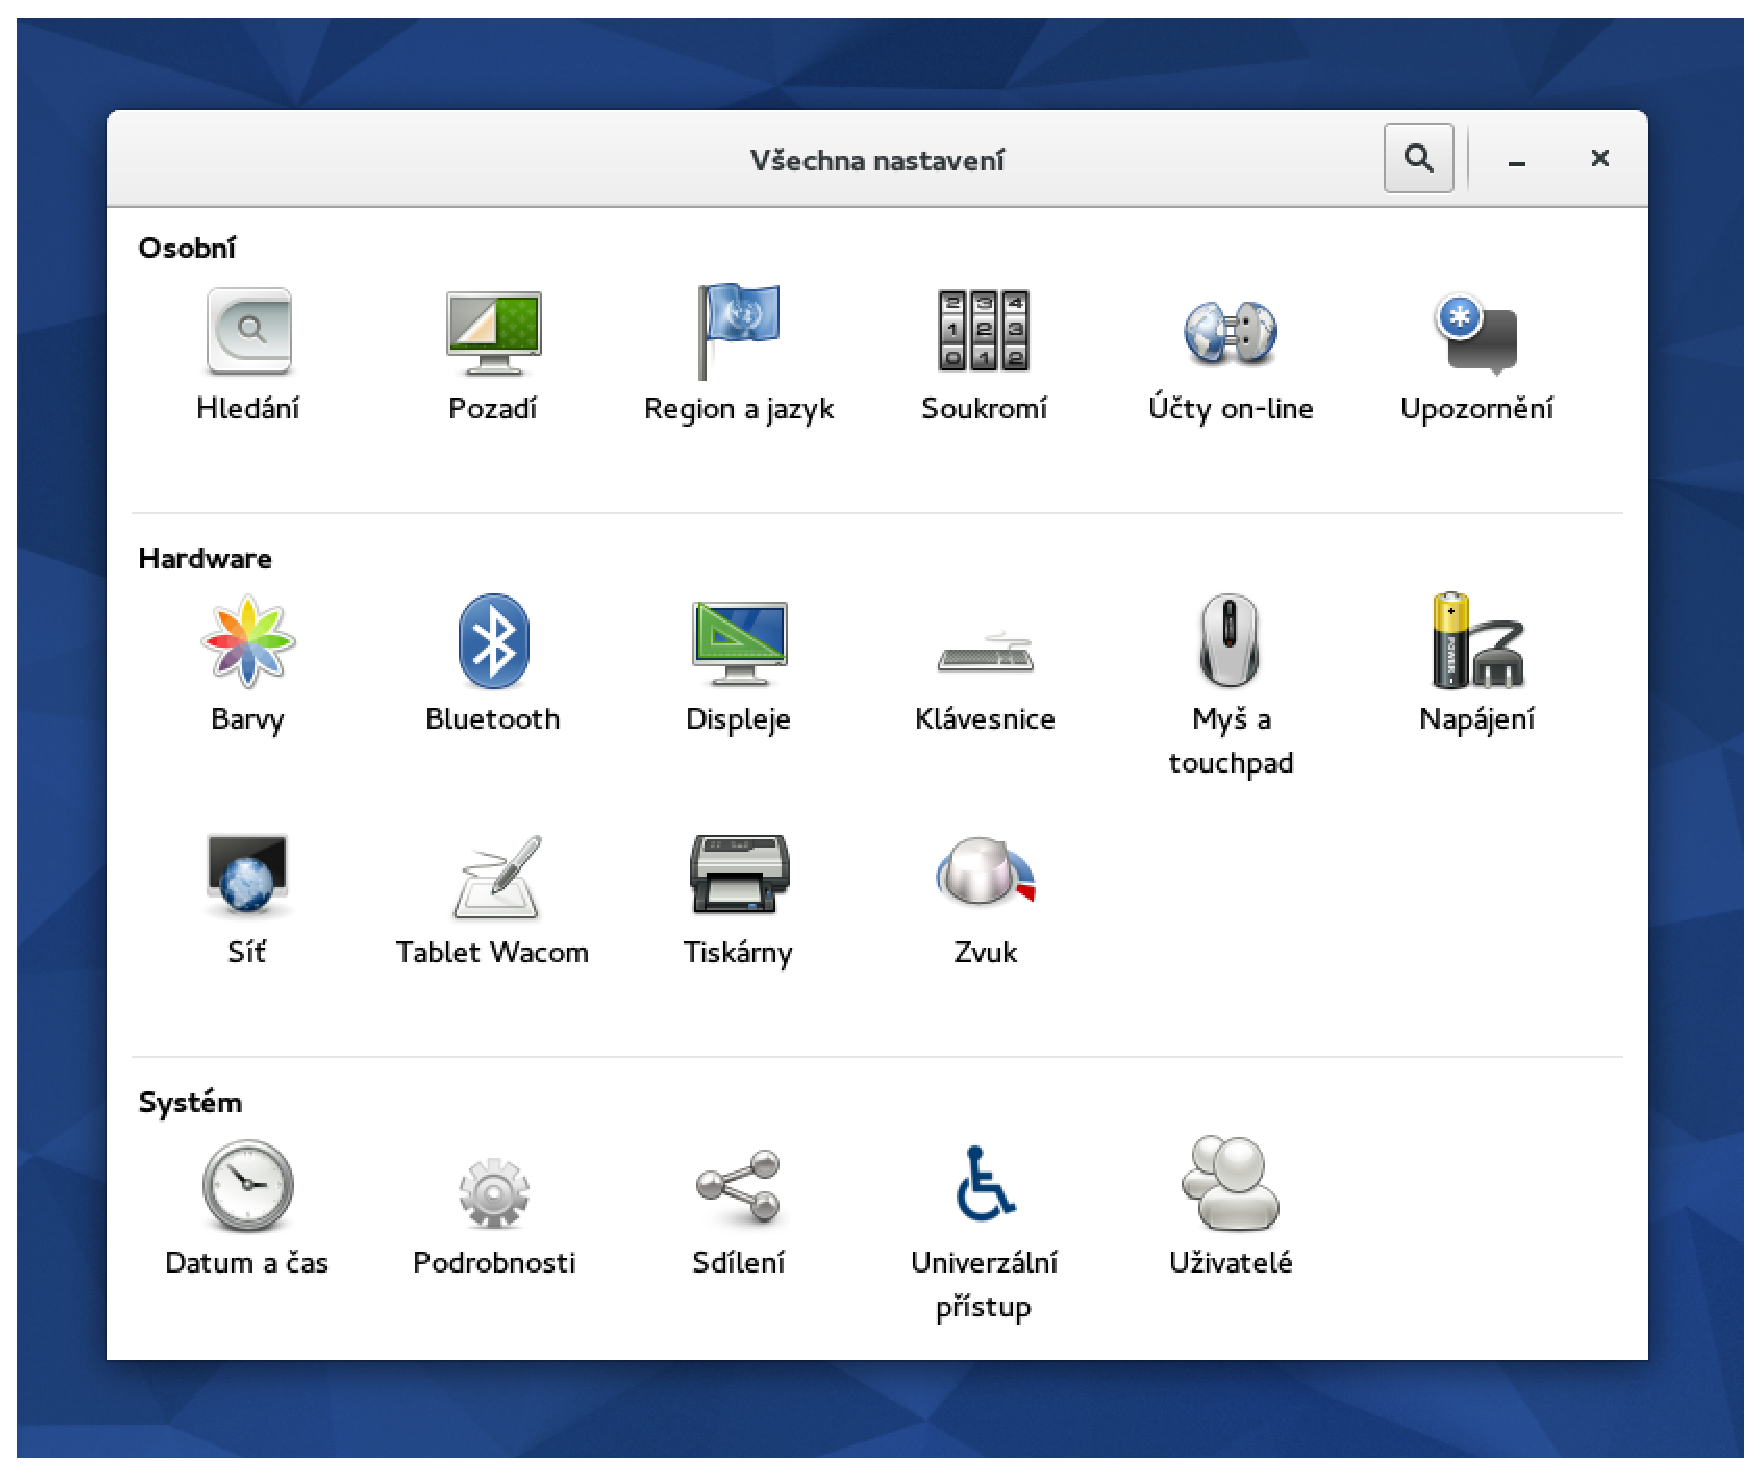
\includegraphics[width=\textwidth]{img/nastaveni}
\captionbelow{nastaveni.} \label{fig:nastaveni}
\end{center}
\end{figure}

\section*{Instalace nového software}
Fedora už v~základu obsahuje mnoho potřebných aplikací (webový prohlížeč \emph{Mozilla~Firefox}, kancelářský balík \emph{LibreOffice}, multimediální přehrávač \emph{Totem} a desítky dalších). Co když ale potřebujeme více programů? Ne všechen software může být zahrnut do výchozí instalace systému, je ale dostupný v~tzv. repozitářích, z~nichž lze daný program jednoduše stáhnout. Repozitář je tvořen sadou serverů a jejich zrcadel, kde jsou umístěny balíky s~různými aplikacemi a knihovnami. Slyšeli jste o~\uv{appstore} na různých mobilních platformách? Pak jste velice blízko, základní princip je stejný. Chcete nějaký program stáhnout z~webu a nainstalovat? Zkuste se nejprve podívat, zda není k~dispozici v~repozitářích. Na Linuxu se tak instaluje naprostá většina aplikací. Jak tedy na to?

\begin{enumerate}
\item \emph{Grafický správce} -- aplikace \emph{Software} je přesně ten druh programu, který znáte z~libovolné mobilní platformy. Je to elegantní a přehledná vstupní brána do repozitářů, kde lze dle názvu (nebo v~rámci kategorie) vyhledávat celistvé aplikace a různé doplňky pro systém. Každá aplikace zde má svůj přehledný popis včetně licence a své velikosti. Stále platí: vše je opensource, vše je bezplatné. Přes nástroj \emph{Software} můžeme aplikace samozřejmě i odinstalovat a setkáme se s~ním vždy, když budeme systém (a balíky v~něm) aktualizovat.

\begin{figure}[t]
\begin{center}
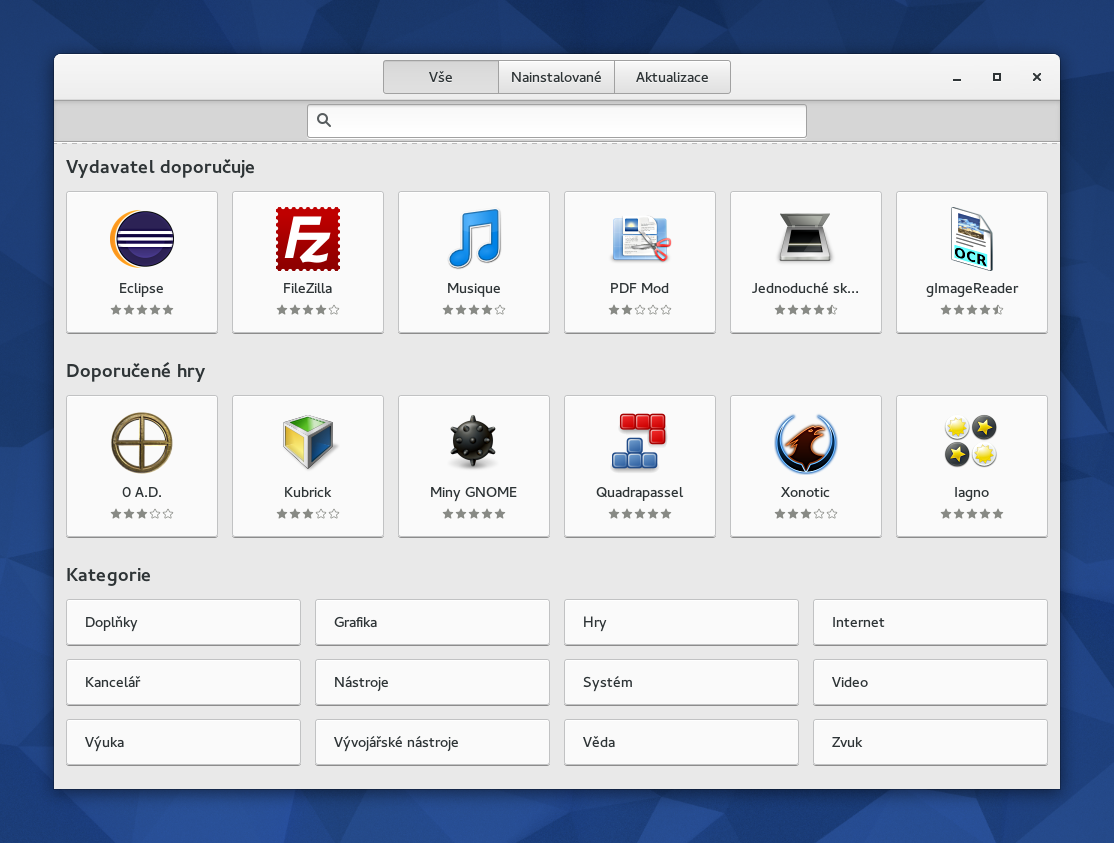
\includegraphics[width=\textwidth]{img/software}
\captionbelow{software.} \label{fig:software}
\end{center}
\end{figure}

\item \emph{Nástroj DNF} -- skrze nástroj \emph{Software} lze v~repozitářích dohledat hlavně ucelené spustitelné aplikace. Není ale určen na dohledání jednotlivé (třeba vývojářské) knihovny, dokumentace nebo různých dílčích utilit. Ve Fedoře je přitom takřka dvacet tisíc balíků, zdaleka ne všechny však obsahují pouze aplikace. Pro přístup ke všem balíkům (a jejich vyhledávání, instalaci, apod.) můžeme použít nástroj \emph{dnf} (určený pro práci v~shellu, není však těžké se jej naučit užívat) nebo jeho nadstavbu \emph{Yum extender (DNF)}, která je opět grafická a dává nám veškerý uživatelský komfort.
\end{enumerate}

\section*{Kodeky a další software}
Co když nějaký software k~dispozici v~repozitářích není? I~taková situace může nastat. Často se jedná o~specifický kodek nebo ovladač. Takový software nemusí být nezbytně placený, může být volně dostupný, ale už ho není (z~licenčních, nebo patentových důvodů) možné zahrnout do Fedory. Tady nastupují repozitáře třetích stran, které nejsou spravované ani jinak spojené s~Fedorou, ale mohou být velmi užitečné. (Dodejme, že za tyto zdroje softwaru nenese Fedora Project zodpovědnost a že nemusí mít vyřešenou právní nezávadnost podle autorského a patentového práva.)

\begin{enumerate}
\item \emph{Firemní repozitáře} -- korporace jako Google nebo Adobe nabízejí zdroje software obsahující jejich produkty. Jsou to různé vývojářské utility, ale i programy jako \emph{Google Chrome}, \emph{Adobe Flash plugin} a další. Jak jednou z~jejich webu nainstalujeme balík přidávající do našeho systému repozitář, vidíme dostupný software v~nástrojích stejně tak jako dříve zmíněný \emph{Software} nebo \emph{dnf}. Obdobným způsobem ho pak také spravujeme.

\item \emph{Další repozitáře} -- existují velké zdroje software třetích stran s~množstvím balíků, ke kterým např. nemáme k~dispozici zdrojové kódy nebo jsou jinak nevyhovující, ale které jsou stále užitečné. Multimediální kodeky a různé specifické ovladače pak můžeme nalézt v~repozitářích jako je (asi nejznámější) \emph{RPMFusion}. Instalace balíků pak opět probíhá analogicky.

\item \emph{Copr repozitáře} -- na rozdíl od předchozích dvou zmíněných variant jsou repozitáře Copr za všech okolností licenčně čisté. Je snadné je přidat a jsou, vedle oficiálních repozitářů, momentálně největší zdroj softwaru pro Fedoru. Může se jednat o~nové verze desktopových prostředí, frameworků apod. Samozřejmě při práci s~nimi je vždy nutné zjistit, co přesně daný software v~systému způsobí. Naleznete je na adrese \url{copr.fedoraproject.org}.

\end{enumerate}
